\documentclass[12pt]{article}
\usepackage[utf8]{inputenc}
\usepackage{fullpage}
\usepackage{color}
\usepackage{listings}
\usepackage{graphicx}
\title{CSC 431 Compiler Report}
\date{}
\author{Austin Wise, Ryan Schroeder}

\begin{document}
\maketitle
\tableofcontents

\pagebreak

\section{Architecture}
\paragraph{}
A small data flow engine hooks all the pieces of the compiler together.
First we parse the command line arguments.
Based on the values we obtain from the argument parser we construct a tree of tasks that represents the actions we want to perform.
The nodes in the tree represent the actions and the edges pass data from one node to its dependants.
Using our Step.DoAll function we execute each step in a topological sorted order, passing the output of each step to the input of the steps that depend on it.

\paragraph{}
The tree of tasks is designed to be run inside of a .NET Task.
A TaskLocal class allows for global variables that have a specific value for each task, similar to thread local storage.
This allows many files to be compiled simultaneously inside one process.
The CompileAllBenchmarks.exe program takes advantage of this to compile all the benchmarks quickly.

\begin{figure}
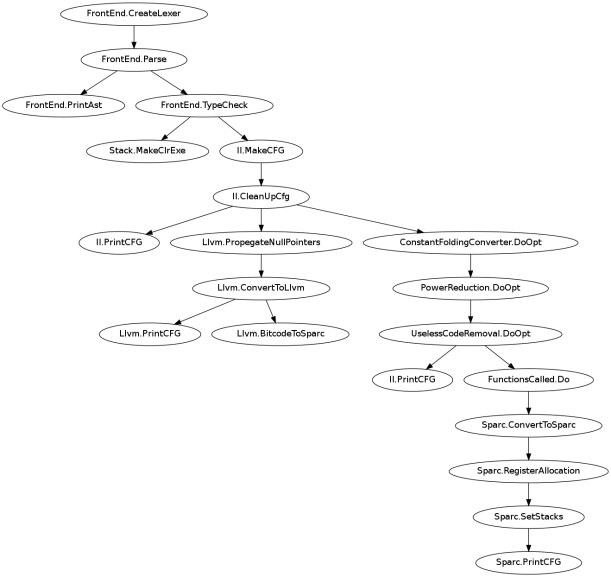
\includegraphics{compSteps.png}
\caption{Tree of tasks created by the compiler.}
\label{compSteps}
\end{figure}


\pagebreak

\section{Representation of Key Data}


\subsection{Instructions}
\paragraph{}
All instruction classes inherit from the abstract Instruction class.
This class has a couple properties, such as the source and destination registers, which allow optimizations and register allocation to be written in a generic way.
There are also abstract instruction classes in the type hierarchy for SPARC, Miloc, and LLVM that carry extra information for those types of instructions.


\paragraph{}
We use the T4 templating engine to generate one class for each instruction.
Each instruction is defined with a single line that gives its name and operands.
Optionally flags can be used to mark an instruction as critical or otherwise change their functionality.
Additionally the templates generate classes and interfaces to aid in the translation of instructions from one type to another (i.e. Miloc to SPARC).

\subsection{Control Flow Graph}
\paragraph{}
All nodes in the control flow graph inherit from the Node class.
The node classes have a generic type parameter that can be used to limit them to holding one type of instruction at a time.
This abstract base class provides information such as a next list and label number to aid in optimizations and printing.
There are subclasses of Node for conditionals, loops, and basic blocks.


\paragraph{}
All nodes have the ability to copy themselves using the Convert function.
The Convert function takes an implementation of the IInstructionConverter interface to convert its instructions.
The IInstructionConverter interface allows for an n:m mapping of instructions.
This facility is used both for converting between instruction types and for doing code transformations on a single instruction type.


\section{Optimizations Implemented}

\subsection{Constant Folding}
\paragraph{}
First we traverse each basic block and we determine if we can find a constant value for the result of an instruction.
As we traverse the basic blocks we store two tables of values: one global table representing instructions that have constant values and a local table.
The local table is constantly being updated with values of registers that are known at the current point in the instruction stream.
When we encounter an unknown instruction we remove all of its destination registers from the local table.
After traversing each block individually we iteratively visit each block again looking for cross block constant expressions until we can find no more.
We use the reaching definitions of the source registers to check if they have a constant value.
The resulting map of instructions to constant values is used by ConstantFoldingConverter (an implementation of IInstructionConverter) to replace the instructions with loads.

\subsection{Power Reduction}
\paragraph{}
We use our IInstructionConverter interface to implement a class that primarily passes through instructions unchanged.
However, when it encounters a multiply or divide instruction whose second argument is a constant value that is a power of two, instead we yield a shift instruction.

\subsection{Useless Code Removal}
\paragraph{}
In our T4 template, important instructions such as returns, branchs, and memory access are defined as critical.
Using reaching definitions we mark all instructions that the critical instructions depend upon.
We then sweep all unmarked instructions by using an IInstructionConverter that skips all marked instructions.

\section{Performance of the Benchmarks}
\subsection{Methodology}
\paragraph{}
We compiled benchmarks with compiler both with and without optimizations.  GCC was also usecd to compile the C version of the benchmarks with -O0 and -O3.
The LLVM and .NET backends do not yet run correctly on SPARC so they are not included in graphs.

  
\end{document}
